%!TeX root=../tese.tex
%("dica" para o editor de texto: este arquivo é parte de um documento maior)
% para saber mais: https://tex.stackexchange.com/q/78101/183146

%% ------------------------------------------------------------------------- %%
\chapter{Conceitos Básicos}
\label{cap:concepts}

Este capítulo apresenta os conceitos que foram utilizados para o desenvolvimento do TCC. Serão apresentadas
as ferramentas utilizadas para realizar o Extract Transform and Load (ETL), simular os logs de ataques, modelos
que foram utilizados e por fim quais frameworks foram usados para a aprendizagem de máquina.

\section{Ferramentas}

\begin{description}
    \item[Kali Linux] \hfill \\ 
        O Kali Linux é uma distribuição linux open source baseada em Debian. 
        Tem como foco auxiliar em tarefas relacionadas a segurança da informação 
        e testes de penetração. \\
        Neste trabalho seus utilitários foram utilizados para simular ataques.
    \item[xsser] \hfill \\ 
        O xsser é um utilitário que está instalado por padrão no kali linux. Sua 
        função é automatizar a deteccão, exploração e análise de ataques XSS em 
        aplicações web. \\
        Ele foi utilizado para gerar requisições HTTP maliciosas que exploram a falha
        XSS.
    \item[sqlmap] \hfill \\ 
        O sqlmap é um utilitário que está instalado por padrão no kali linux. Sua
        função é automatizar a detecção e exploração de ataque de SQL injection em 
        aplicações web. \\
        Ele foi utilizado para gerar requisições HTTP maliciosas que exploram a falha
        de SQL Injection.
    \item[Pandas] \hfill \\ 
        O Pandas é uma ferramenta  em python para o processo de análise de dados, 
        especificamente neste trabalho, foi utilizado para realizar o ETL e análise 
        dos logs coletados.
    \item[DVWA] \hfill \\ 
        DVWA é uma aplicação web com falhas de segurança conhecidas que podem ser 
        exploradas no ambiente local e controlado, facilitando assim a simulação de
        ataques. \\ 
        Aqui foi utilizado para simular um ambiente que tenha as falhas de segurança 
        necessárias e com isso conseguimos gerar os logs necessários para o projeto.
  \end{description}

\section{Modelos de aprendizagem de máquina}

\begin{description}
    \item[Árvore de decisão] \hfill \\ Árvore de decisão é um modelo de representação 
    dos dados que visa classificar os dados tendo como base um conjunto 
    de atributos. \\ 
    Elas são construidas particionando os dados em conjuntos, chamados de nós, 
    até que uma folha seja encontrada. Esta então é a classe do dados. Veja na Figura \ref{fig:ex_decision_tree} 
    em que é mostrada uma árvore de decisão que decide se um aluno está apto a se formar ou não. 
    Nela, os quadrados são os nós e as elipses são as folhas, isto é, a respectiva classe do 
    dado.
    \begin{figure}
        \centering
        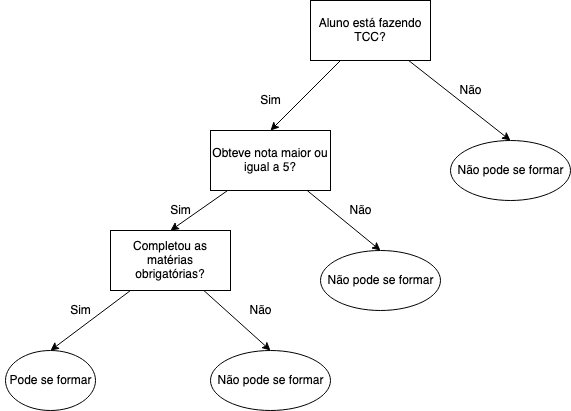
\includegraphics[width=.8\textwidth]{figuras/ex_decicion_tree1.png}
        \caption{Exemplo de árvore de decisão.\label{fig:ex_decision_tree}}
    \end{figure}

    Este modelo é útil pois a sua interpretabilidade é alta. A intrepretabilidade é grau com que 
    um modelo pode ser entendido em termos humanos. 
    
    Por exemplo, quando comparado com o modelo de florestas aleatórias que utiliza várias 
    árvores de decisão para realizar a classificação, entender como cada árvore influência 
    na classificação final dificulta a interpretabilidade no contexto geral, portanto,
    o modelo de árvore de decisão ter um interpretabilidade maior do que o de florestas de decisão.

    \item[Florestas aleatórias] \hfill \\ Florestas aleatórias é um modelo de aprendizagem 
    de máquina que combina árvores de decisão. Isto é, uma certa quantidade de árvores são 
    treinadas de maneira independente uma da outra, utilizando diferentes partes do conjunto de 
    dados. \\ 
    E para realizar a classificação, cada árvore realiza uma classificação (voto) e o resultado 
    final da floresta é a classe com mais votos, como ilustrado na image Figura \ref{fig:ex_random_forest}
    que apresenta uma floresta aleatória, onde a árvore 1 utliza o conjunto de características $N_1$ 
    para realizar a classificação que resulta na classe C, a árvore 2 utliza o conjunto de características $N_2$ 
    para realizar a classificação D, e assim por diante. E a classe final é a classe B pois é a que 
    possui a maior quantidade de votos: \\

    \begin{figure}
        \centering
        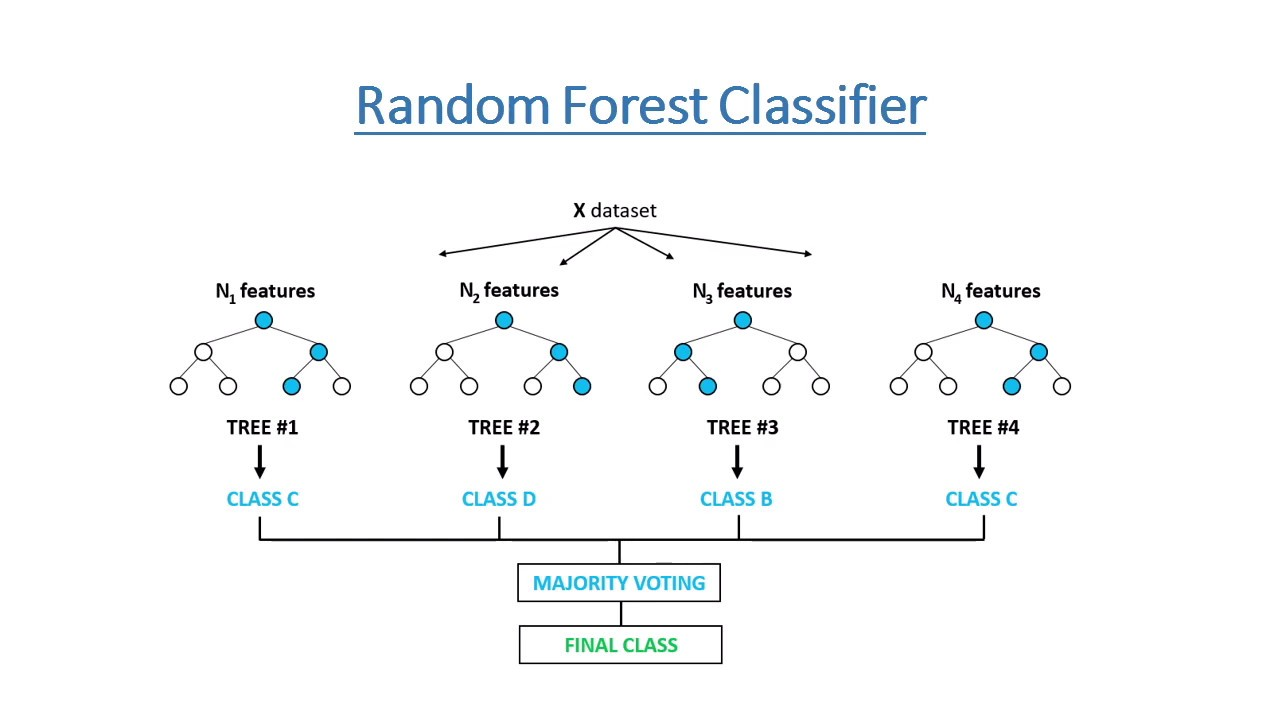
\includegraphics[width=.9\textwidth]{figuras/ex_random_forest.jpg}
        \caption{Exemplo de floresta aleatória, retirado do trabalho \cite{ref:imagem_random_forest} \label{fig:ex_random_forest}}
    \end{figure}

    Este modelo possui dois pontos de atenção: sua interpretabilidade é baixa, dado o número de 
    classificadores que temos que analisar, e também é consideravelmente mais pesado que o anterior, 
    pois ele treina algumas árvores de decisão e não apenas uma.
\end{description}

\section{Ferramentas de aprendizagem de máquina}

\begin{description}
    \item[scikit-learn] \hfill \\ Scikit-learn é uma ferramenta que implementa algoritmos de aprendizagem
    de máquina, supervisionados e não supervisionados. Em particular, o modelo de árvore de decisão e floresta
    aletória.\\ 
    Além disso, ela integra com o ecossistema python, isto é: numpy, pandas e matplotlib. E também 
    fornece uma interface sólida, que facilita o seu uso.  \\
    Neste trabalho foi usado para treinar, avaliar e selecionar quais modelos foram utilizados 
    para executar os experimentos.

    \item[Apache Spark] \hfill \\ Apache Spark é uma ferramenta para trabalhar com aprendizagem 
    de máquina de maneira distribuida ou em um único nó. \\
    Assim como o scikit-learn, há alguns modelos implementados que estão prontos para serem utilizados, 
    em particular, há implementações de árvore de decisão e floresta aleatória. \\
    Há suporte para algumas linguagens, como: Python, Scala, Java e R. \\
    Neste trabalho foi usado para executar os experimentos com o modelo selecionado.
\end{description}

\section{Segurança em servidores HTTP}

\begin{description}
    \item[Ataque XSS] \hfill \\ Ataque XSS consiste em que scripts maliciosos são injetados em 
    websites confiáveis. Em geral, isso se da por meio de formulários em websites. \\ 
    Este ataque foi um objeto de estudo deste trabalho.
    \item[SQL Injection] \hfill \\ SQL Injection consiste em enviar consultas modificadas a banco 
    de dados por meio de entradas do usuário, com por exemplo campos de texto em forumários, as quais 
    podem ler informação sensiveis do banco de dados as quais tal usário não possue acesso. \\
    Este ataque foi um objeto de estudo deste trabalho.
    \item[Registro de acessos nos logs] \hfill \\ Nos registros de acceso de logs são armazenadas as
    informações de um requisição HTTP, neles podemos encontrar dados com o endereço IP de origem,
    data e hora e endereço requisitado, para citar alguns dados.  \\
    Neste trabalho, esses registros foram utilizados como fonte primária de dados para treinar 
    e validar os modelos de aprendizagem de máquina.
\end{description}

\section{Outros conceitos}

\begin{description}
    \item[Extract Transform and Load (ETL)] \hfill \\ ETL é o processo de extrair, transformar 
    e carregar dados de uma fonte de dados de origem para outr de destino. Nesse processo, 
    características podem ser adicionadas, valores discrepantes removidos e padrões aplicados,
    para citar algumas operações comuns. \\ 
    Neste trabalho foi utilizado para transformar os arquivos de logs do formato original para 
    o formato tabular, que são usados nas ferramentas de aprendizagem de máquina.
    \item[Virtualização] \hfill \\ Virtualização é o processo de executar multiplas intâncias 
    de sistemas operacionas em uma abstração do mesmo hardware. Com isso é possivel 
    criar instâncias isoladas de sistemas operacionais em um mesmo computador. \\
    Neste trabalho, foi utilizado para criar as instancias vítima e atacante.
    \item[Notebooks] \hfill \\ Notebook são arquivos divididos em células que executam
    trechos de código Python. Ele facilita a experimentação pois guarda os resultados das
    células, evitando assim a necessidade de executar o mesmo trecho de código multiplas
    vezes. \\ 
    Neste trabalho foi utilizado para realizar ETL, além de treinar e validar os modelos
    de aprendizagem de máquina. 
\end{description}